\documentclass[12pt, a4paper]{article}

\usepackage{fancyhdr}
\usepackage[left=4cm, right=4cm, top=4cm, bottom=4cm]{geometry}
\usepackage[utf8]{inputenc}
\usepackage[table]{xcolor}
\usepackage{hyperref}
\usepackage{amsmath}
\usepackage{enumitem}
\usepackage{graphicx}
\usepackage{booktabs}
\usepackage{subcaption}
\usepackage[justification=centering]{caption}
\usepackage{xepersian}

\DeclareMathOperator*{\argmax}{argmax}
\DeclareMathOperator*{\argmin}{argmin}
\newcolumntype{L}{>{$}l<{$}} % math-mode version of "l" column type

\newcommand{\coursetitle}{پردازش زبان طبیعی}
\newcommand{\doctitle}{تمرین سوم}
\newcommand{\name}{محمدرضا غفرانی}
\newcommand{\studentno}{400131076}
\newcommand{\todaydate}{\today}

\settextfont{XB Kayhan}
\setlatintextfont{Times Newer Roman}

\pagestyle{fancy}
\lhead{\textbf{\doctitle}}
\chead{\name}
\rhead{\todaydate}

\begin{document}

\begin{flushleft}
    \name \\
    \studentno \\
    \todaydate
\end{flushleft}

\begin{center}
    \huge
    \textbf{\coursetitle}
    \break
    \large
    \doctitle
\end{center}

% suppress the fancy header on the first page only
\thispagestyle{plain}

\section*{سوال یک}

در انجام این سوال نکات زیر ملاحظه شده است.

\begin{itemize}
    \item با توجه به آن که کتابخانه \lr{Bert Embedding} بر روی تعداد کلمات ورودی محدودیت می‌گذاشت بنابراین
    ما \lr{context} هر کلمه هدف را با ده کلمه قبل و بعد آن ساخته و به مدل دادیم. در قدم بعدی تعبیه کلمه
    هدف از بردار‌های ارائه شده مدل استخراج می‌شود.
    \item در مجموعه داده‌ای که در اختیار ما قرار داده شده بود ناسازگاری‌هایی وجود داشت. مثلا برای کلمه \lr{hard}
    تنها یک معنی در مجموعه داده آموزشی گزارش شده بود، یا مثلا برای کلمات دیگر معانی پرت گزارش شده بود.
    در نهایت ما برحسب صورت تمرین و داده‌های موجود در مجموعه دادگان طبق جدول زیر معانی را نظر گرفتیم.
    (جدول \ref{word_meaning})

    \begin{latin}
        \begin{table}[h]
            \caption{\rl{جدول معنای کلمه در مجموعه دادگان}}
            \label{word_meaning}
            \begin{tabular}{c|c}
                Word & Meaning \\
                \hline
                hard & HARD1, HARD2, HARD3 \\
                interest & interest1, interest2, interest3, interest4, interest5, interest6 \\
                line & division, cord, phone, formation, product, text \\
                serve & SERVE10, SERVE12
            \end{tabular}
        \end{table}
    \end{latin}

    \item از آن جا که برای کلمه \lr{hard} در مجموعه داده آموزشی و آزمون پس از انجام
    \break پیش‌پردازش‌های بالا تنها یک معنی وجود دارد،
    بنابراین بر روی آن صحت و \lr{F1} برابر ۱۰۰ گزارش شده است.

    \item برای هر کلمه به صورت جداگانه \lr{SVM} آموزش داده شده است. در هنگام گزارش معیار \lr{F1}
    به دلیل وجود برچسب‌های مختلف، معیار \lr{F1} برای هر برچسب جداگانه محاسبه شده و با استفاده از \lr{macro-averaging}
    نتایج ارائه شده است.
\end{itemize}

نتایج زیر بر اساس پیش‌پردازش‌های توضیح داده شده تولید شده است. لازم به ذکر است که برای به دست آوردن بهترین
خروجی پارامتر‌های مختلفی نظیر کرنل و مقدار $C$ برای دسته‌بند \lr{SVM} بررسی شده است. نتایج زیر با استفاده از
کرنل \lr{Linear} و مقدار $C=1$ ارائه شده است. (جدول \ref{svm_without_val})

\clearpage

\begin{latin}
    \begin{table}[h]
        \centering
        \caption{\rl{عملکرد دسته‌بندی \lr{SVM} در مجموعه داده}}
        \label{svm_without_val}
        \begin{tabular}{c|c|c|c|c}
            & \multicolumn{2}{c|}{train} & \multicolumn{2}{c}{test} \\
            \hline
            Word & Acc & F1 & Acc & F1 \\
            \hline
            hard     & 1 & 1 & 1 & 1 \\
            interest & 1 & 1 & 0.94 & 0.822 \\
            line     & 1 & 1 & 0.948 & 0.947 \\
            serve    & 1 & 1 & 1 & 1
        \end{tabular}
    \end{table}
\end{latin}

\section*{سوال دو}

نکاتی در رابطه با پیاده‌سازی انجام شده ذکر می‌شود.

\begin{itemize}
    \item برچسب‌های در نظر گرفته شده برای هر کلمه همانند توضیحات داده شده در صورت سوال است.
    با توجه به آن که طول بزرگترین جمله موجود در مجموعه دادگان ۱۴۱ بود، ما فرض کردیم بیشترین
    وابستگی موجود بین ۱۳۰ کلمه سمت راست و ۱۳۰ کلمه سمت چپ باشد. بر طبق همین فرض در یک بازه
    پیوسته تمامی برچسب‌هایی که نشان‌دهنده وابستگی تا حداکثر ۱۳۰ کلمه سمت راست و ۱۳۰ کلمه سمت چپ هستند
    را تولید می‌کرده و در نظر می‌گیریم.
    \item ما مسئله را به صورت یک مسئله دسته‌بندی حل کرده‌ایم. یعنی مدل برای هر کلمه یک برچسب از برچسب‌های
    موجود در مجموعه زیر را انتخاب کرده و خروجی می‌دهد.

    $$\{\texttt{<ROOT>}, \texttt{<1R>}, \texttt{<2R>}, ..., \texttt{<129R>}, \texttt{<1L>},
    \texttt{<2L>}, ..., \texttt{<129L>}\}$$

    \item از مدل \lr{wrod2vec} ارائه شده توسط گوگل که با نام \lr{word2vec-google-news-300}
    معروف است به عنوان مدل تعبیه کلمه استفاده کرده‌ایم. با توجه به آن که تعداد کلمات موجود در این مدل
    بسیار زیاد است (حدود ۳ میلیون)، بنابراین برای جلوگیری از مصرف بی‌ازحد حافظه تنها ۵۰۰ هزار کلمه
    آن استفاده شده است. این مجموعه داده برای هر کلمه یک بردار ۳۰۰ بعدی ارائه می‌دهد.
    \item طول جمله‌ها با حاشیه‌گذاری عدد $0$ یکسان شده است. از آن که طول بزرگترین جمله
    برابر ۱۴۱ است، در حالی که اکثر جملات دارای طول ۶۰ هستند بنابراین حجم بسیاری از مجموعه داده
    را همین حاشیه‌گذاری تشکیل می‌دهد. مدل با پیش‌بینی همین مقادیر حاشیه‌گذاری شده می‌تواند به دقت‌های
    خوبی برسد. برای جلوگیری از این موضوع در هنگام آموزش شبکه از تابعی استفاده شده است تا مقادیر
    صفر در مقدار صحت نهایی دخیل نشود. در هنگام گزارش مقادیر دقت، بازیابی و \lr{F1} این مقادیر
    حذف شده است.
    \item برای محاسبه معیار‌های صحت، دقت، بازیابی و \lr{F1} از جدول درهم‌ریختگی با حذف سطر و ستون متناظر
    \lr{padding} استفاده شده است. معیار‌های دقت و بازیابی با میانگین‌گیری \lr{macro} به ازای
    سطر‌ها و ستون‌هایی که دارای مقدار بودند به دست آمده است. معیار \lr{F1} با استفاده از دقت و بازیابی
    کلی که محاسبه می‌شود محاسبه شده است.
\end{itemize}

حال به ارائه نتایج می‌پردازیم. ما از دو شبکه مختلف برای ارائه نتایج بهره برده‌ایم. یک شبکه همان
شبکه توصیف شده در صورت سوال است و شبکه دیگر از دو لایه شبکه \lr{LSTM} تشکیل شده است. این دو لایه
به صورت پشته روی هم قرار گرفته‌اند. بین هر دو شبکه \lr{LSTM} یک لایه \lr{Dropout} با مقدار $0.2$
در نظر گرفته شده است. نتایج این دو مدل در جدول زیر آورده شده است.

\begin{latin}
    \begin{table}[h]
        \centering
        \caption{\rl{مقایسه عملکرد شبکه‌ عصبی پیجیده‌تر در مقایسه با شبکه ساده‌تر}}
        \label{complex_vs_simple}
        \begin{tabular}{c|c|c|c|c|c|c|c|c}
                    & \multicolumn{4}{c|}{validation} & \multicolumn{4}{c}{test} \\
            \hline
            Model & Acc & Prec & Rec & F1 & Acc & Prec & Rec & F1 \\
            \hline
            Simple & 0.764 & 0.381 & 0.200 &  0.263 & 0.765 & 0.324 & 0.169 & 0.222 \\
            Complex & 0.822 & 0.568 & 0.344 & 0.428 & 0.825 & 0.529 & 0.338 & 0.412
        \end{tabular}
    \end{table}
\end{latin}

همان‌طور که مشاهده می‌شود مدل دوم توانسته‌ است نتایج بهتری را ارائه دهد. بنابراین
به نظر می‌رسد پشته‌کردن کردن و استفاده از لایه‌های \lr{Dropout} مفید واقع شده باشد.
هدف از ارائه کردن لایه \lr{Dropout} این بود که هر بار بخشی از خروجی شبکه
از بین برده شود تا مدل سعی کند با همان توانایی محدود‌تر نتیجه بگیرد. بدین ترتیب
مدل خروجی بهتری را تولید می‌کند. با توجه به یکسان بودن عملکرد مدل به ازای
بار‌های مختلف اجرا می‌توان گفت این نتایج قابل اتکا است.

در تحلیل نتایج ارائه شده به ازای معیار‌های مختلف می‌توان گفت که معیار \lr{Accuracy} اعداد قابل
قبولی را برای هر دو مدل ارائه داده است. اما سایر معیار‌ها از نظر عددی خوب نیستند. برای توجیه دلیل این
اتفاق می‌توان گفت که چون میانگینی که برای ادغام نتایج دسته‌های مختلف انجام شده است، به صورت غیر وزن‌دار
انجام شده است، بنابراین نتایج مدل به ازای کلاس‌هایی نظیر \lr{\texttt{<10L>}} که تعداد کم‌تری داشته‌اند
در مقایسه با کلاس‌های \texttt{<ROOT>} با هم جمع زده و میانگین گرفته می‌شود. بنابراین عملکرد ضعیف مدل
در کلاس‌ها با داده کم‌تر (که مدل به خوبی آن‌ها را نیاموخته است) موجب ارائه نتایج ضعیف برای معیار‌های
\lr{Precision} و \lr{Recall} می‌شود.

علت بالاتر بودن عدد گزارش‌ شده برای \lr{Precision} هم آن است که چون در \lr{Precision} برخی از کلاس‌ها
اصلا تولید نشده است، بنابراین از میانگین حذف شده است اما در \lr{Recall} همه این کلاس‌ها در
نقش داده و در نتیجه بین تعداد بیشتری میانگین گرفته شده است.

در ادامه نمودار
خطای آموزش برای هر دو مدل آورده می‌شود.

\begin{figure}[h]
    \centering
    \begin{subfigure}{0.45\linewidth}
        \centering
        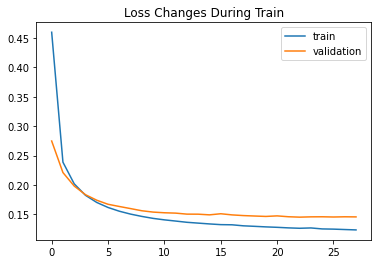
\includegraphics[width=0.8\linewidth]{images/loss1.png}
        \caption{نتایج مدل ساده}
    \end{subfigure}
    \begin{subfigure}{0.45\linewidth}
        \centering
        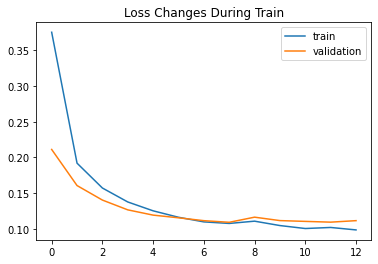
\includegraphics[width=0.8\linewidth]{images/loss2.png}
        \caption{خطای مدل پیچیده‌تر}
    \end{subfigure}
    \caption{نمودار خطای آموزش و ارزیابی در گام‌های یادگیری}
\end{figure}

در نهایت درخت وابستگی برای نمونه‌هایی که در فایل تمرین قرار داده شده است، آورده می‌شود.
این نتایج با استفاده از مدل پیچیده‌تر که نتایج بهتری دارد ارائه شده است.

\clearpage

\begin{figure}[t]
    \centering
    \begin{subfigure}{0.9\linewidth}
        \centering
        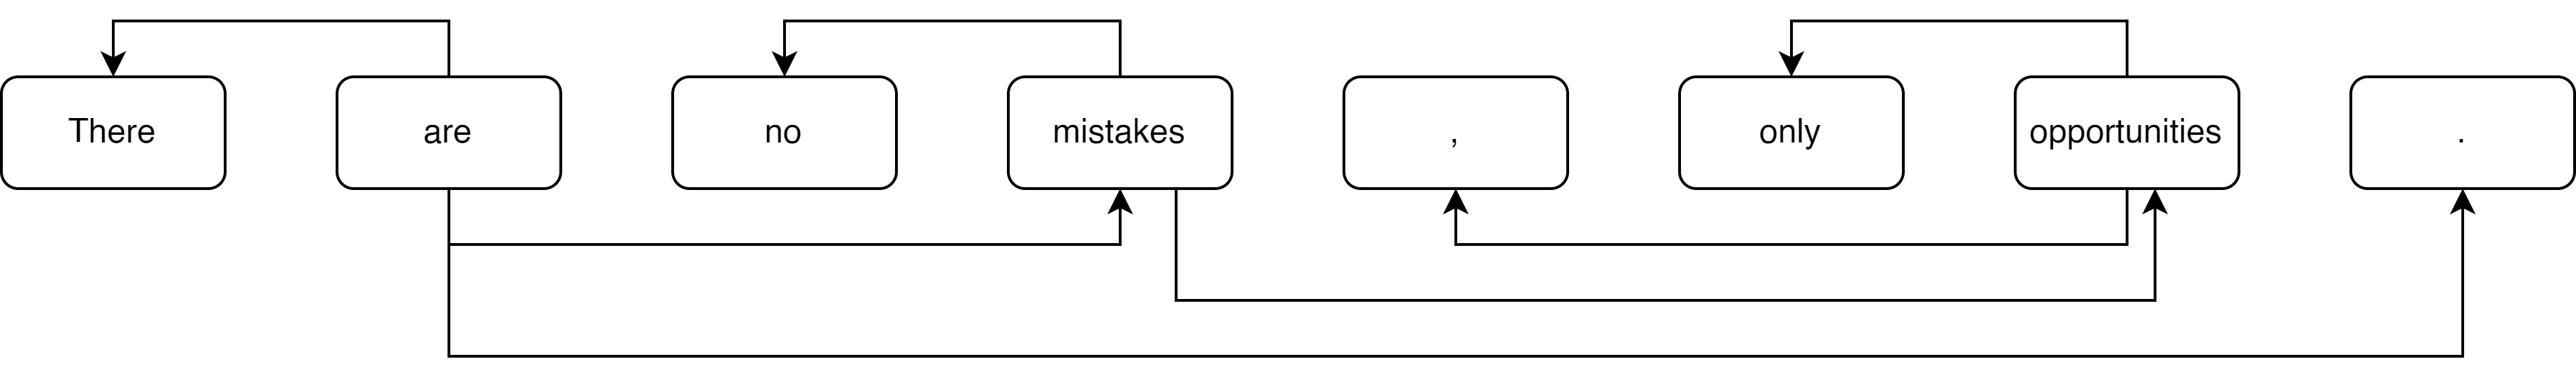
\includegraphics[width=0.8\linewidth]{images/s1.png}
        \caption{\lr{There are no mistakes, only opportunities.}}
    \end{subfigure}
    \centering
    \begin{subfigure}{0.9\linewidth}
        \centering
        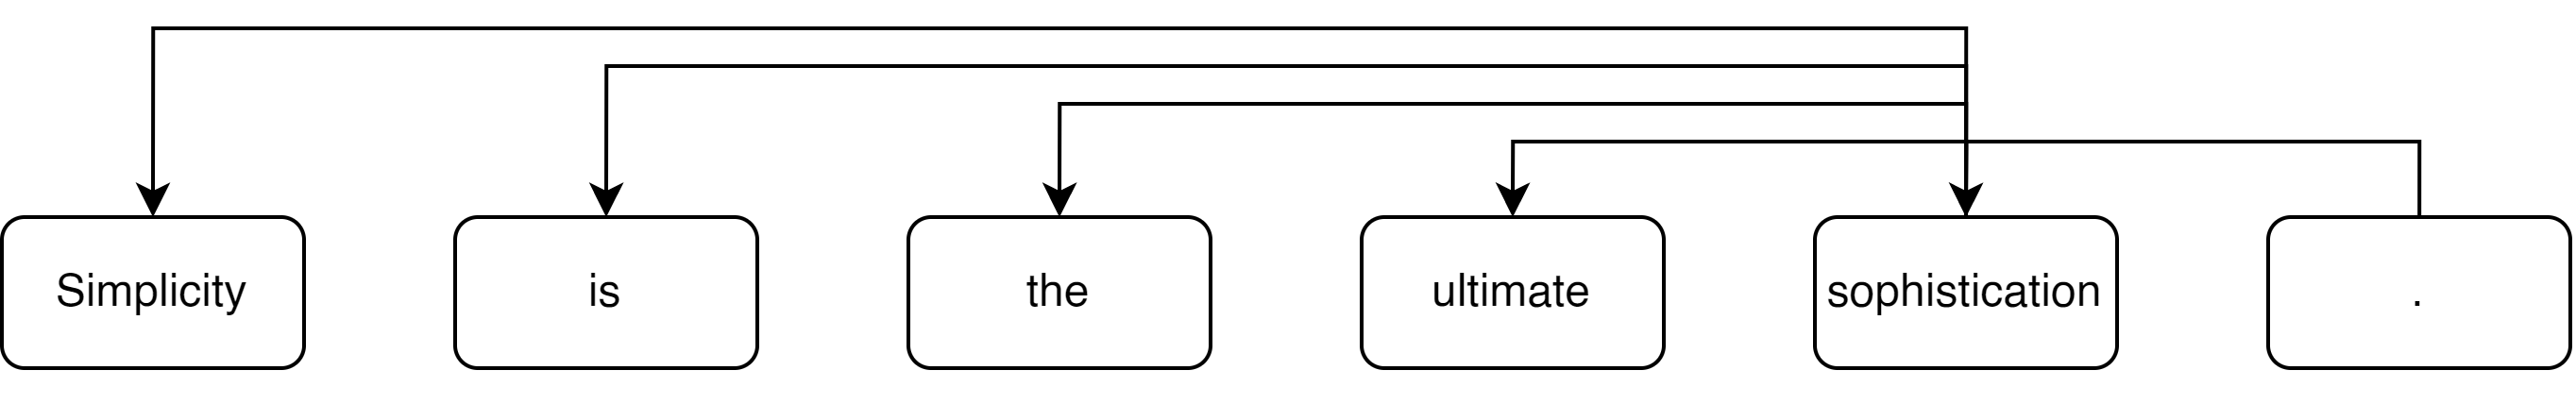
\includegraphics[width=0.8\linewidth]{images/s2.png}
        \caption{\lr{Simplicity is the ultimate sophistication.}}
    \end{subfigure}
    \begin{subfigure}{0.9\linewidth}
        \centering
        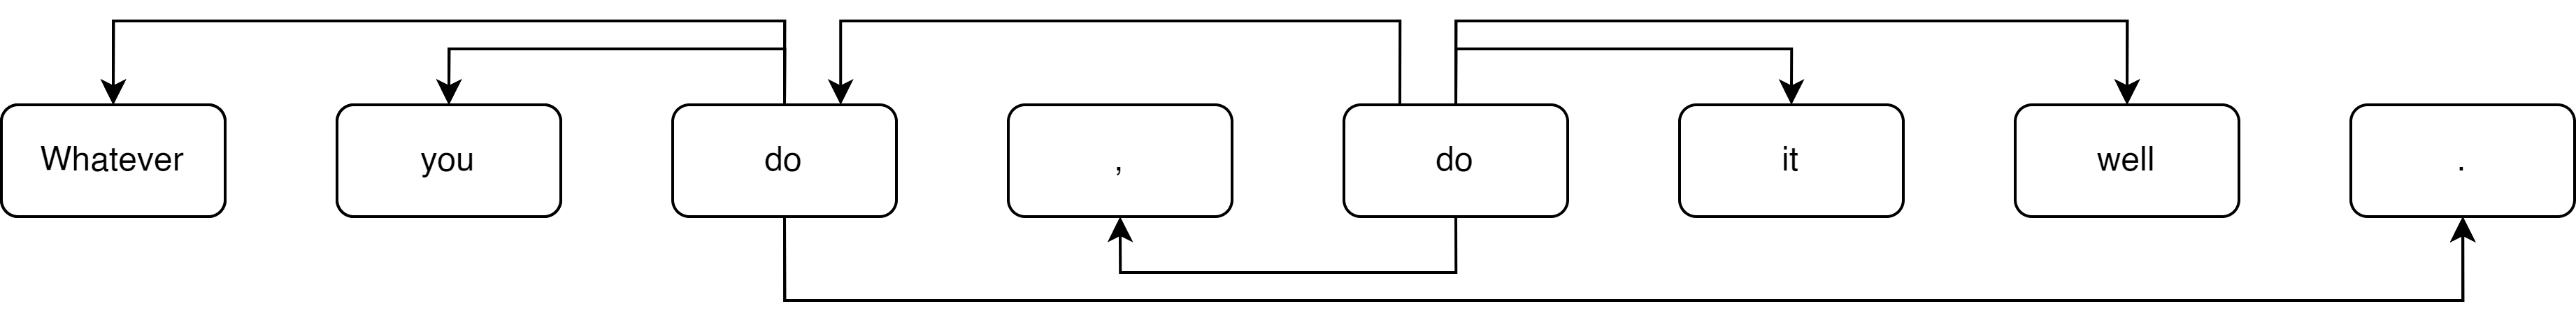
\includegraphics[width=0.8\linewidth]{images/s3.png}
        \caption{\lr{Whatever you do, do it well.}}
    \end{subfigure}
    \caption{خروجی‌های مدل پیچیده برای جملات داده شده}
\end{figure}



\end{document}